\documentclass[border=10pt]{standalone}
\usepackage[svgnames]{xcolor}
\usepackage{amsmath}
\usepackage{pgfplots}
\pgfplotsset{compat=newest}
\usepackage[sfdefault]{FiraSans}
\usepackage{FiraMono}
\renewcommand*\familydefault{\sfdefault}
\begin{document}
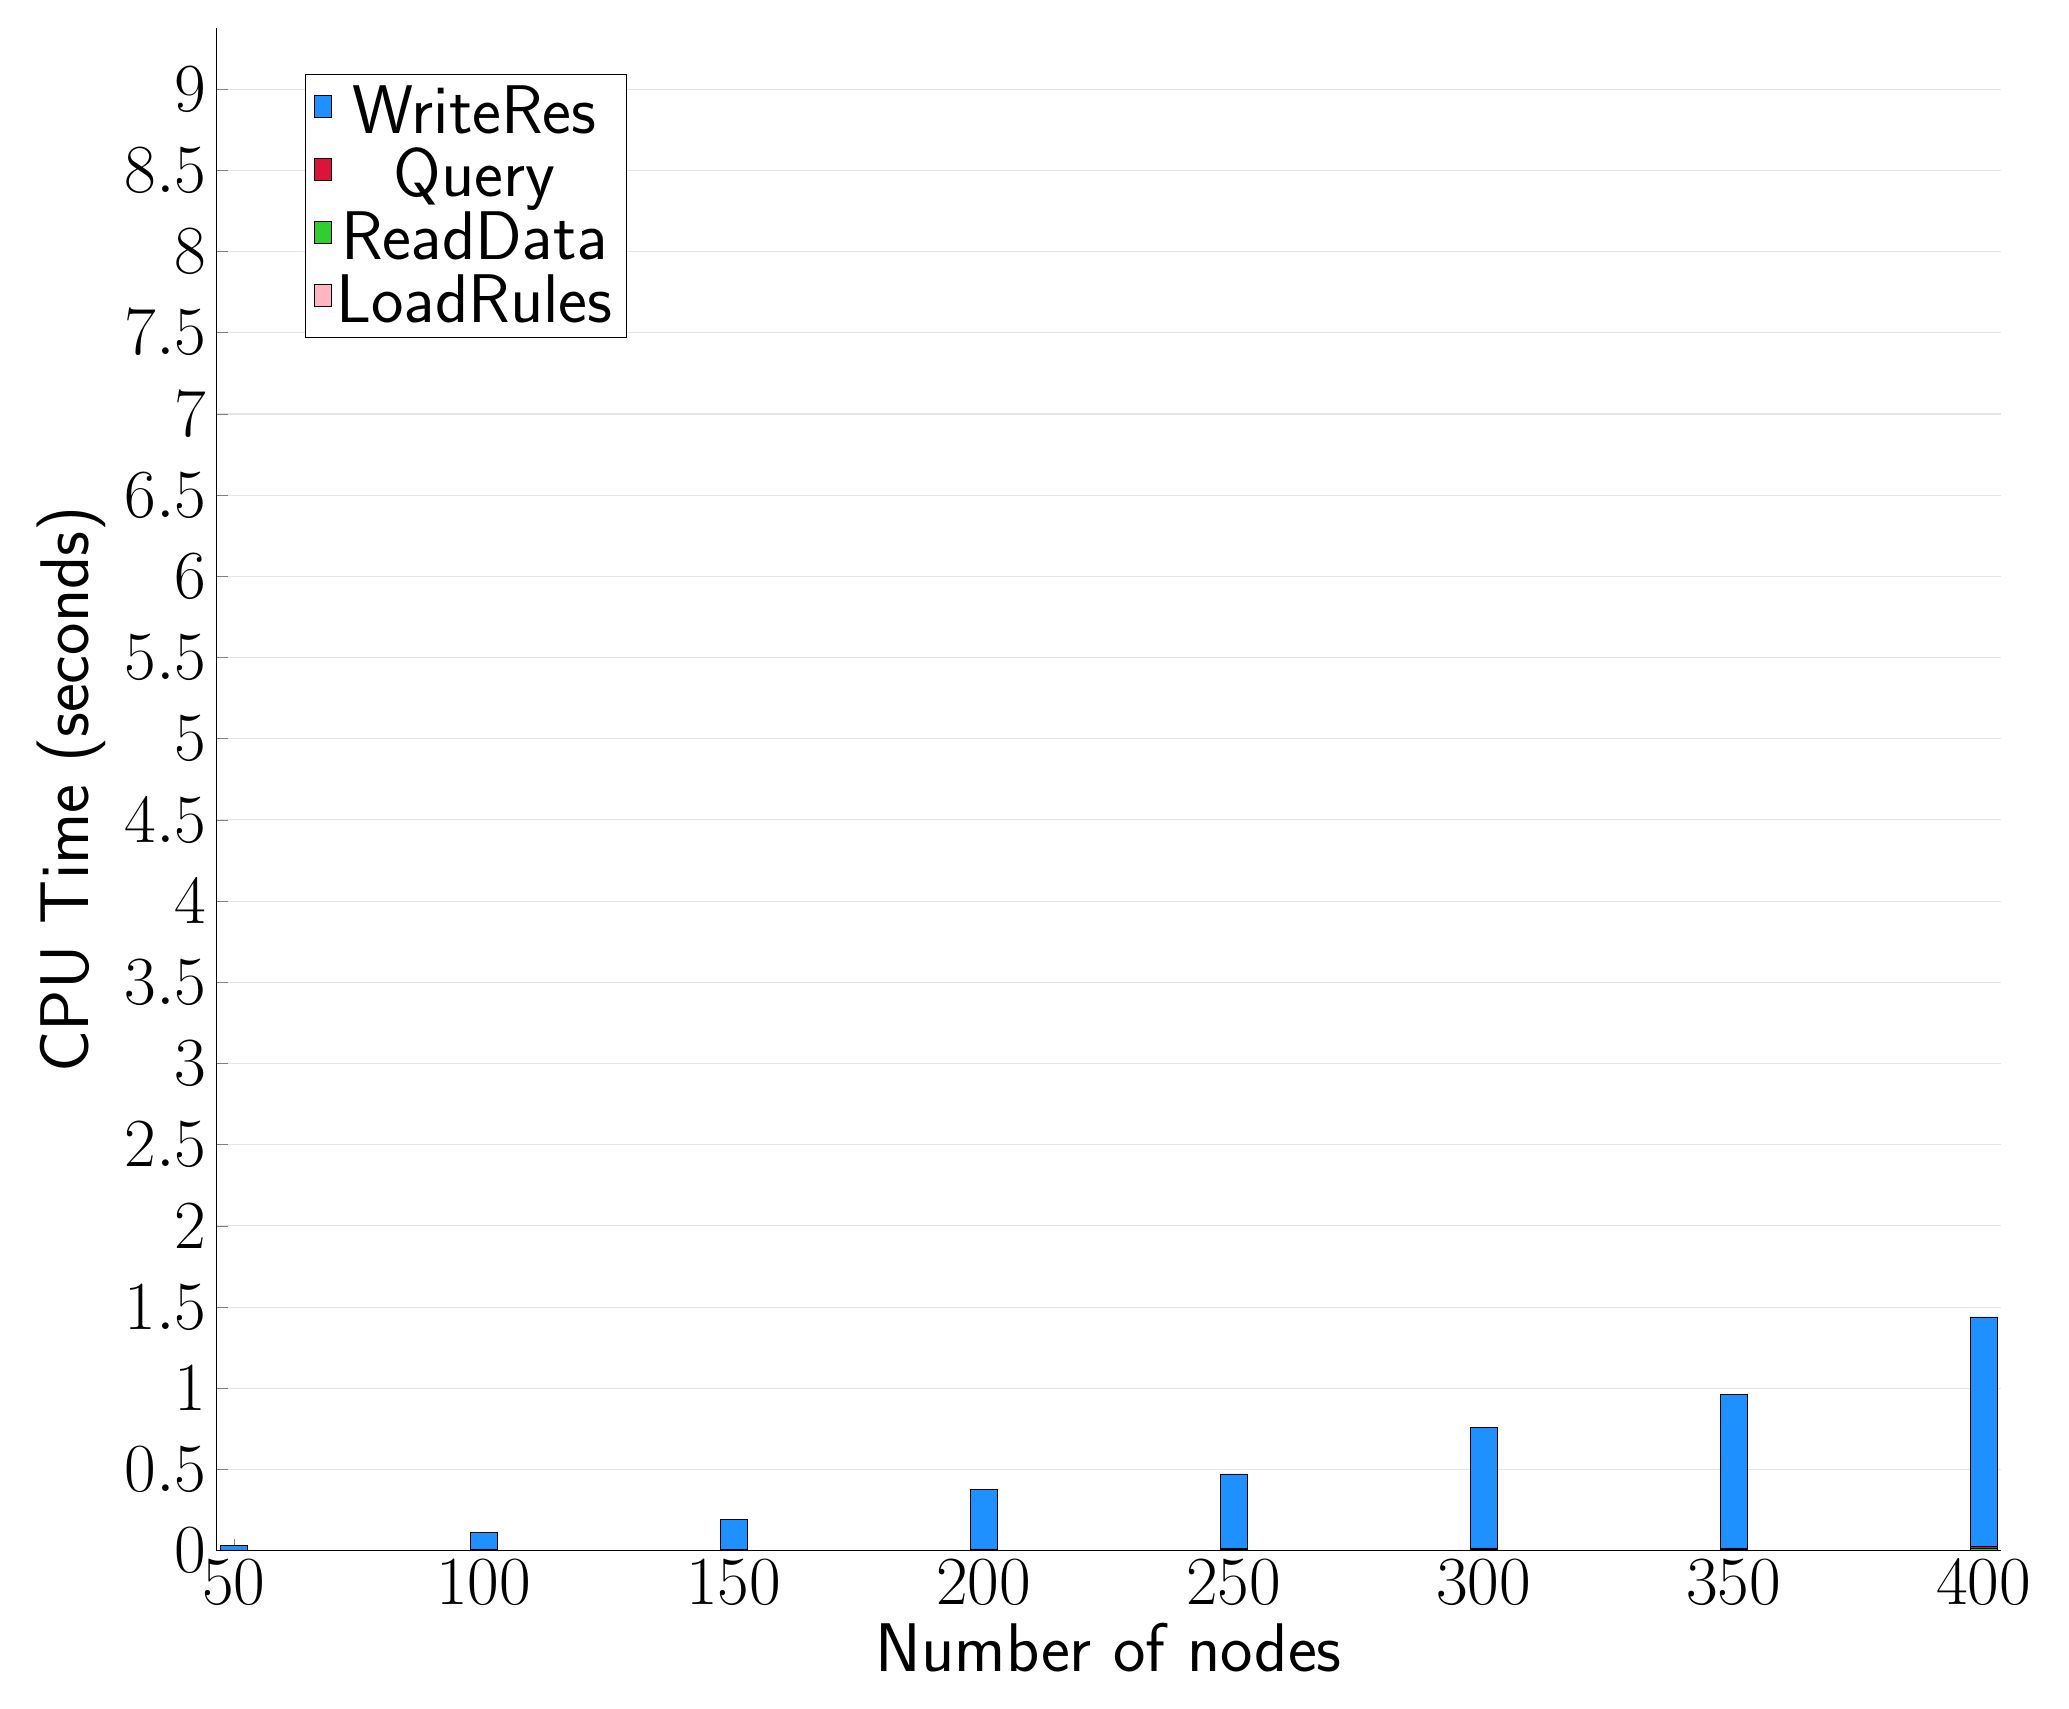
\begin{tikzpicture}
\begin{axis}[
   ybar stacked,
   width=2\textwidth,
   bar width=0.35cm,
   ymajorgrids, tick align=inside,
   major grid style={draw=gray!20},
   xtick=data,
   ymin=0, ymax=9.375487327575684,
   axis x line*=bottom,
   axis y line*=left,
   enlarge x limits=0.01,
   legend style={
       at={(0.23, 0.97)},
       anchor=north east,
       legend columns=1,
       font=\Huge,
   },
   ylabel={CPU Time (seconds)},
   xlabel={Number of nodes},
   label style={font=\Huge},
   tick label style={font=\Huge},
]
\addlegendimage{fill=DodgerBlue, draw=black, line width=0.2pt}
\addlegendentry{WriteRes}
\addlegendimage{fill=Crimson, draw=black, line width=0.2pt}
\addlegendentry{Query}
\addlegendimage{fill=LimeGreen, draw=black, line width=0.2pt}
\addlegendentry{ReadData}
\addlegendimage{fill=LightPink, draw=black, line width=0.2pt}
\addlegendentry{LoadRules}
\addplot +[fill=LightPink, draw=black, line width=0.2pt] coordinates {
(50, 0.0032619999999999997)
(100, 0.004002999999999997)
(150, 0.002957333333333333)
(200, 0.003335)
(250, 0.0028476666666666667)
(300, 0.002731666666666667)
(350, 0.0025189999999999965)
(400, 0.003548666666666667)
};
\addplot +[fill=LimeGreen, draw=black, line width=0.2pt] coordinates {
(50, 0.0016506666666666633)
(100, 0.0031773333333333337)
(150, 0.003193333333333333)
(200, 0.004514000000000003)
(250, 0.005553)
(300, 0.00616)
(350, 0.006779333333333329)
(400, 0.008534666666666668)
};
\addplot +[fill=Crimson, draw=black, line width=0.2pt] coordinates {
(50, 0.00030633333333333234)
(100, 0.001236666666666671)
(150, 0.0016990000000000032)
(200, 0.0036329999999999995)
(250, 0.004687333333333333)
(300, 0.00755733333333333)
(350, 0.008103)
(400, 0.013977333333333333)
};
\addplot +[fill=DodgerBlue, draw=black, line width=0.2pt] coordinates {
(50, 0.028153333333333336)
(100, 0.10407366666666668)
(150, 0.18631799999999998)
(200, 0.363882)
(250, 0.4597076666666667)
(300, 0.744996)
(350, 0.9466123333333334)
(400, 1.414103)
};
\end{axis}
\end{tikzpicture}

\end{document}
